\documentclass[11pt,a4paper]{article}
\usepackage[margin=2.2cm]{geometry}
\usepackage{graphicx,booktabs,amsmath}
\newcommand{\arcsec}{$^{\prime\prime}$}
\title{TESS planet candidate around TIC 219396153}
\author{Isak Paulo de Andrade Ruas \\ NROLABS}
\date{\today}
\begin{document}
\maketitle

\section*{Summary}
Signal found by the bls search of a public-data TESS pipeline
(SPOC 120\,s PDCSAP light curves, sectors 87).
Final tier: \textbf{candidate: likely planet}.
Catalogue cross-match (TOIs, CTOIs, published planets, SPOC TCEs, TESS eclipsing binaries):
\textbf{TOI 7888.01} (TOI).
CNN score (calibrated): 0.928.
TRICERATOPS (10 Monte Carlo runs, mean $\pm$ error of the mean):
FPP $= 0.155 \pm 0.0069$,
NFPP $= 0$.

\section*{Host star (TIC v8)}
\begin{tabular}{ll}\toprule
RA, Dec (deg) & 77.838671, -49.357726 \\
TESS magnitude & 13.6 \\
Radius ($R_\odot$) & 0.642 $\pm$ 0.0193 \\
$T_{\rm eff}$ (K) & 3859 $\pm$ 157 \\
Density ($\rho_\odot$) & 2.35 $\pm$ 0.135 \\
Distance (pc) & 220 \\\bottomrule
\end{tabular}

\section*{Transit fit}
Limb-darkened model (quadratic law, Kipping $q_1,q_2$; GPU float64, 1024 annuli, 1024x4096 tables, 15x supersampling), emcee with 48 walkers,
12000 steps (802 burn-in), run until the chain exceeded 50 autocorrelation times.
Medians and 68\% intervals.

\begin{tabular}{lc}\toprule
Mid-transit time $T_0$ (BJD$_{\rm TDB}$) & $2460668.7548^{+0.0036}_{-0.0035}$ \\
Period $P$ (days) & $10.2370^{+0.0038}_{-0.0034}$ \\
Radius ratio $R_p/R_\star$ & $0.0950^{+0.0096}_{-0.0074}$ \\
Impact parameter $b$ & $0.49^{+0.28}_{-0.32}$ \\
Stellar density $\rho_\star$ (g cm$^{-3}$) & $2.2^{+1.2}_{-1.3}$ \\
Limb darkening $q_1$ & $0.50^{+0.32}_{-0.30}$ \\
Limb darkening $q_2$ & $0.48^{+0.33}_{-0.31}$ \\
Depth (ppm) & $10518^{+1129}_{-1091}$ \\
Duration $T_{14}$ (hours) & $3.32^{+0.33}_{-0.25}$ \\
$a/R_\star$ & $23.0^{+3.5}_{-5.6}$ \\
Inclination (deg) & $88.8^{+0.8}_{-1.3}$ \\
Planet radius ($R_\oplus$) & $6.66^{+0.71}_{-0.56}$ \\
Semi-major axis (au) & $0.069^{+0.011}_{-0.017}$ \\
Equilibrium temperature (K, $A=0$) & $572^{+84}_{-48}$ \\
Insolation ($S_\oplus$) & $18^{+13}_{-5}$ \\
\bottomrule\end{tabular}

\section*{Vetting}
\begin{tabular}{lccc}\toprule
Test & Value & Pass condition & Result \\\midrule
Transit SNR (correlated noise) & 9.63 & $\ge 7.1$ & pass \\
Transits observed & 2 & $\ge 2$ (periodic) & pass \\
Odd/even depth difference ($\sigma$) & -- & $\le 4$ & pass \\
Secondary eclipse ($\sigma$) & 2.59 & $\le 3.9$ & pass \\
Ingress fraction (V shape) & 0.242 & $\le 0.4$ & pass \\
Planet radius ($R_\oplus$) & 7.19 & $\le 25$ & pass \\
Centroid source offset (arcsec) & 4.21 & 4$\sigma$ and $>$21\arcsec & pass \\
Difference image offset (arcsec) & -- & 4$\sigma$ and $>$10.5\arcsec & pass \\
Difference image significance ($\sigma$) & -- & -- & -- \\
CCD common mode ($\sigma$) & -0.542 & $\le 4$ & pass \\
Crowding (CROWDSAP) & 0.994 & $\ge 0.8$ & pass \\
Stellar density ratio (max/TIC) & 0.974 & $\ge 0.2$ & pass \\
\bottomrule\end{tabular}

\section*{Caveats}
\begin{itemize}
\item This is a candidate with statistical evidence, not a confirmed planet: confirmation needs high-resolution imaging, reconnaissance spectroscopy and radial velocities.
\item TRICERATOPS was run without a high-resolution imaging contrast curve, so close bound companions are not excluded.
\item The MCMC converged (chain longer than 50 autocorrelation times, stable estimate) (acceptance 0.18, 12000 steps, about 3342 independent samples); errors are scaled by the time-averaging factor $\beta = 1.18$ for correlated noise.
\item Stellar radius and effective temperature come from TIC v8; if the TIC gives no error, 7\% (radius) and 150 K were assumed.
\end{itemize}

\begin{figure}[h!]\centering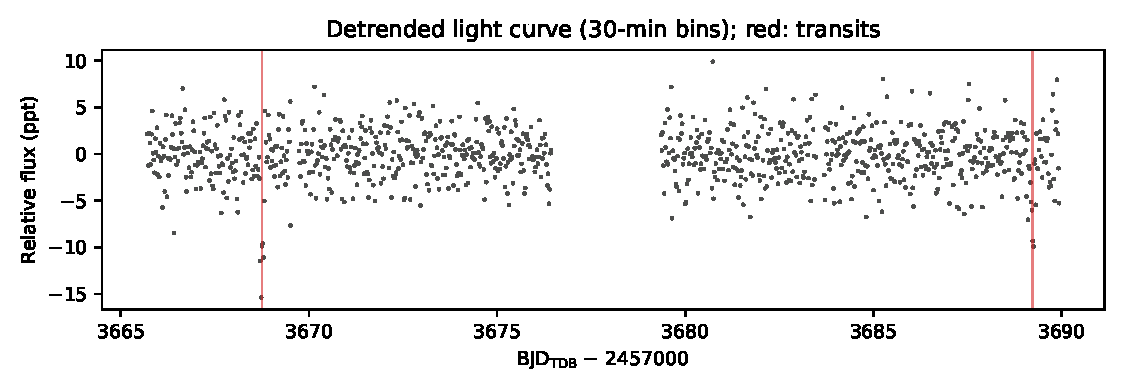
\includegraphics[width=1\textwidth]{lightcurve.pdf}\caption{Detrended SPOC PDCSAP light curve (transit-protected biweight).}\end{figure}
\begin{figure}[h!]\centering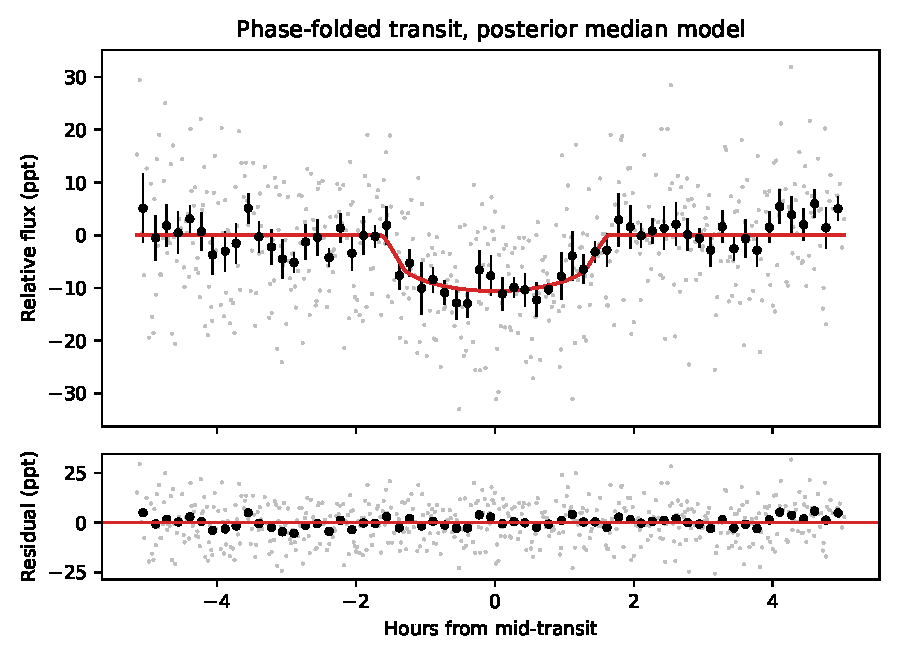
\includegraphics[width=.8\textwidth]{folded.pdf}\caption{Phase-folded transit with the posterior median limb-darkened model.}\end{figure}
\begin{figure}[h!]\centering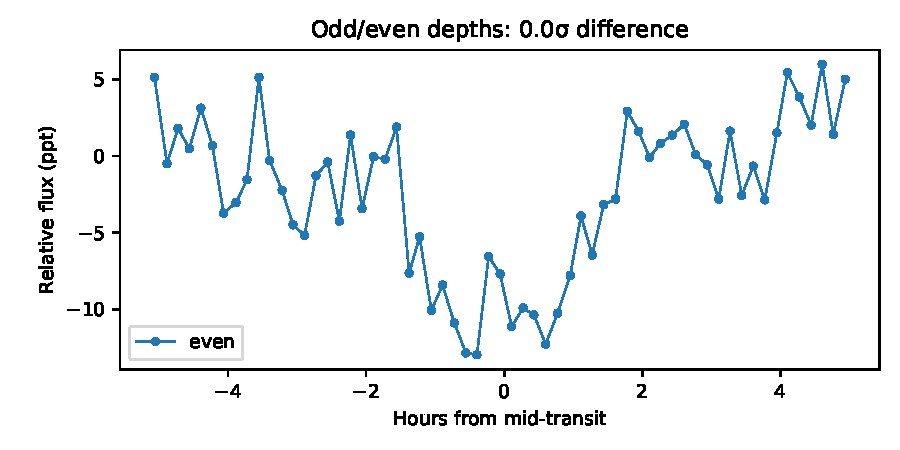
\includegraphics[width=.7\textwidth]{odd_even.pdf}\caption{Odd and even transits, binned to 10 minutes.}\end{figure}
\begin{figure}[h!]\centering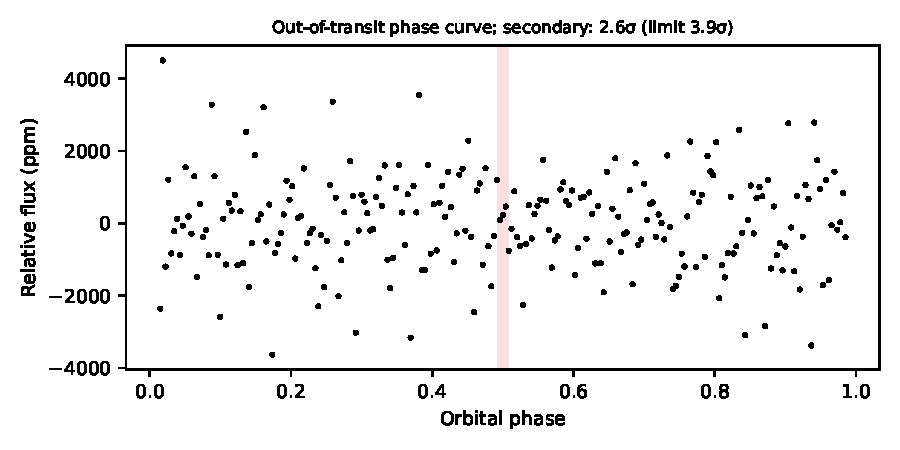
\includegraphics[width=.7\textwidth]{secondary.pdf}\caption{Phase curve; the shaded band is the secondary eclipse window for a circular orbit.}\end{figure}
\begin{figure}[h!]\centering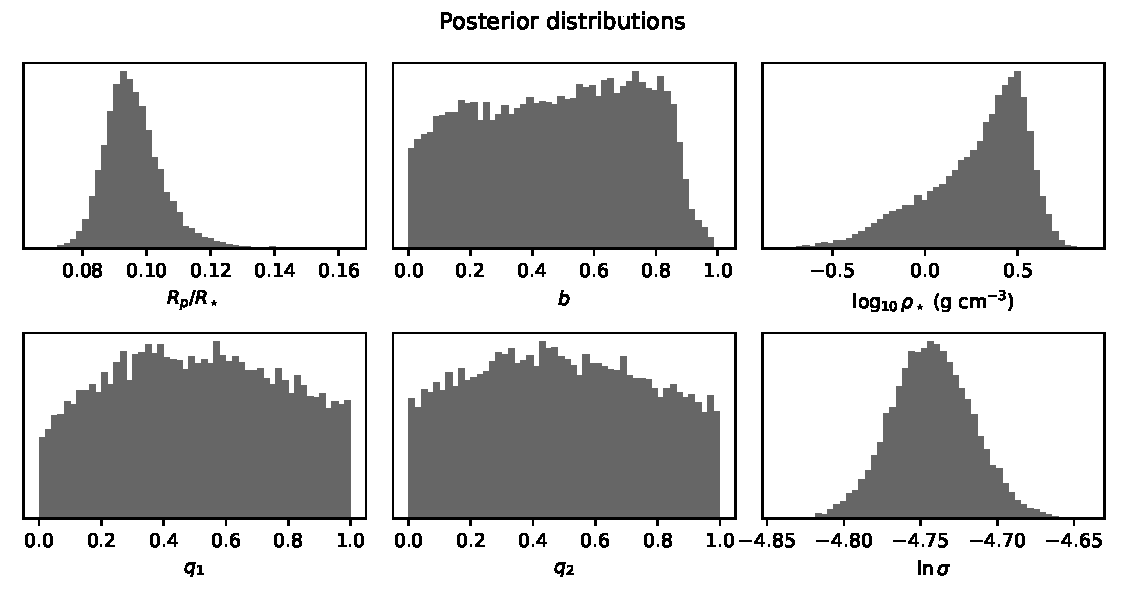
\includegraphics[width=.9\textwidth]{posterior.pdf}\caption{Posterior distributions of the fitted parameters.}\end{figure}
\end{document}
